\documentclass[sigconf]{acmart}

\setcopyright{none}
\settopmatter{printacmref=false} % Removes citation information below abstract
\renewcommand\footnotetextcopyrightpermission[1]{} % removes footnote with conference information in first column

\theoremstyle{definition}
\newtheorem{definition}{Definition}[section]
\DeclareMathOperator*{\argmax}{argmax}

\usepackage{algorithm} 
\usepackage{algpseudocode} 
\DeclareMathOperator{\sign}{sign}

\usepackage{pgfplots}
\pgfplotsset{compat=1.15}
\usepackage{mathrsfs}
\usetikzlibrary{arrows}

\begin{document}

%%
%% The "title" command has an optional parameter,
%% allowing the author to define a "short title" to be used in page headers.
\title{Query recommendation system \\
    \large Data Mining Project 2022/2023}

%%
%% The "author" command and its associated commands are used to define
%% the authors and their affiliations.
%% Of note is the shared affiliation of the first two authors, and the
%% "authornote" and "authornotemark" commands
%% used to denote shared contribution to the research.
\author{Erik Nielsen}
\email{mat. 238755}
\affiliation{
  \institution{University of Trento}
  \city{38123 Povo TN}
  \country{Italy}
}
\email{erik.nielsen@studenti.unitn.it}


\author{Fabrizio Sandri}
\email{mat. 238825}
\affiliation{
  \institution{University of Trento}
  \city{38123 Povo TN}
  \country{Italy}
}
\email{fabrizio.sandri@studenti.unitn.it}


\begin{abstract}

Since the birth of computing, there's always been discussion on how an information system can be used to recommend a product to a customer based on his interests. From the first practical application for a system called Grundy \cite{grundy}, a computer-based library that recommended novels to the users based on their interests, recommendation systems have gained wider attention thanks to the widespread diffusion of internet. Nowadays, these systems are fundamental to the user experience inside web services and social networks. In many cases, recommendation systems are the reason why one service is preferred over another.

This research explores a strategy that begins by identifying similar queries using solely LSH with collaborative filtering, then employs a hybrid algorithm that combines both collaborative filtering and content-based techniques to get more accurate recommendations. The results indicate that our method may produce valuable query recommendations, indicating that it has the potential to be used in real-world scenarios. 

\end{abstract}
\pagestyle{plain}

%%
%% This command processes the author and affiliation and title
%% information and builds the first part of the formatted document.
\maketitle

\section{Introduction}

In the past decade, data has become ubiquitous, and as a result, the need to store large amounts of data in an efficient way has become increasingly important. Databases have emerged as the preferred method for organizing and storing information in an organized and efficient way. Since the 1970s, most database management systems have been designed around the relational model\cite{relational_model} where the most fundamental elements that characterize it are relations, commonly referred to as tables. A relation is a collection of tuples, or table rows, each of which shares a set of characteristics, or table columns. The most typical method of retrieving data from a DBMS is to send a query, or a structured request for a set of data. 

Let's suppose that we have access to a large number of queries that each user submits to a database management system (DBMS), each of which is associated with a rating that indicates how satisfied the user is with the query's outcome. In particular, let's assume that our DBMS is made up of a single relation that allows users to submit multiple queries to retrieve data. The question that remains is whether we can exploit all of this data to suggest queries to users based on previous interests. 

% Why you think that such a study is important? 
Making recommendations is essential in many fields, starting with e-commerce websites where these systems attempt to suggest the best products that match the user's interest in order to improve sales. This methodology is used in e-commerce as well as libraries, as in the case of the aforementioned Grundy system. Another scenario is when streaming services try to find the movie that aligns most with a user's preferences.

%Introduction to the recommendation system
These systems are usually based on the so-called \emph{Utility Matrix}, which captures a user's preference for a particular item offered by the service. The matrix itself has some blank spaces, as usually users don't have recorded data about each item of the system. So the goal of the recommendation systems is to provide meaningful values for the blank spaces inside the matrix.


% why it is challenging (i.e., not trivial) to perform this processing? What were the hard/challenging parts in developing a solution?
There is an infinite amount of ways to create a recommendation system, starting with the two fundamental approaches: content based and collaborative filtering. These are not the only ones; in fact, clustering is another option that can be taken into account while looking for groups of commonalities that can suggest one thing to another member of the same group. Each of these approaches must cope with the problem of dealing with huge amount of data and finding the best recommendation in the shortest amount of time; in most of the cases, it shouldn't take more than a few seconds to find a good recommendation, as is the case with e-commerce websites where the customer can see recommendations right away. In general, making recommendations based on massive volumes of data is still a challenging research problem. 

% introduction to databases and query and the problem statement
As recommendation systems are mainly based on already existing data, the presence of some sort of database is necessary for the workflow of the algorithm.
These databases are usually based on the relational model and thus organized in tables made of rows and columns, built with the purpose to have an easy architecture and more understandable data. This paper first demonstrate how locality sensitive hashing can be used to improve similar items search to provide user recommendations, and then shows how the incorporation of a content-based approach to build a hybrid recommendation system may be beneficial for the recommendations' accuracy. 

\section{Related work}

The work that has been conducted so far in the field of recommendation systems has been focused on finding ways to exploit similarities in existing data to make recommendations. This prior knowledge can take on a variety of shapes; one well-known form is provided in terms of a utility matrix. It can also be obtained from other sources of information that draw on patterns that exploits similarities, such as user behaviours \cite{user_behaviour_rec}. 


Depending on the kind of prior knowledge the system has regarding the problem that is being attempted to solve, there are primarily two categories in which recommendation systems can be categorized; these methods are \emph{content-based filtering} and \emph{collaborative-filtering}. In addition to these two methods in the last few years emerged the necessity to combine the benefits of the two aforementioned methods into \emph{hybrid recommendation systems}.

% intro to content based
Content-based methods use a combination of the features associated with each product and the ratings given by each user to provide suggestions. This method requires the construction of user profiles that outline each user's preferences as well as item profiles that highlight an item's key features. 

% Intro to collaborative filtering
The collaborative-filtering method pushes the system to only consider the relationships between users and items, ignoring either the features of users or the characteristics of items: with this approach, the utility matrix's relationships are the sole thing being considered. It is possible to create collaborative-filtering recommendation systems by either locating similar items that may be of interest based on the user's past interests, this is called \emph{item-item collaborative filtering}, or by utilizing user similarities to recommend products that another user has rated highly, this is \emph{user-user collaborative filtering}; in both cases the similarity of items and users is determined by the similarity of the ratings given by one users to an item. 

% Short intro to hybrid methods
Collaborative filtering and content-based approach can be combined together to produce an hybrid recommendation systems, which aim to combine the advantages of both the approaches to provide recommendations that are even more accurate. Depending on the type of problem being considered, different combining strategies may be used \cite{user_behaviour_rec}.  

% Utility matrix formal definition
As was already anticipated, the fundamental component of a recommendation system is the kind of prior knowledge provided for a particular problem that enables the algorithm to make reasoning about the given information. In the case of recommendation systems the prior knowledge is commonly embedded in a so called \emph{utility matrix}. Given a set of users $U$ and a set of items $I$, the utility matrix can be formally represented by an \emph{utility function} $f$ that associates users $u \in U$ and items $i \in I$ to a rating $r \in R$, where $R$ is a set of valid ratings, i.e. $f: U \times I \to R$.


\subsection{Similarity measures} \label{similatrity_measures}
% short introduction to the similarities measures
The concept of similarity is crucial to the system regardless of the technique chosen to provide recommendations.  In recent years, data mining research has taken into account the issue of selecting appropriate similarity measurement methods as another crucial and effective aspect in the quality of results. According to the literature \cite{similarity_approaches}, similarity measures depend on the problem at hand, which means that although one measure may perform well for one data structure, it might be worse with another structure. 

% Jaccard similarity
\subsubsection{Jaccard similarity}\label{similarity_measure_jaccard}
The \emph{Jaccard similarity}, often referred to as the Jaccard index, is a well established method to measure the similarity between sets. The similarity of two given sets $A$ and $B$, can be measured as the intersection of the sets divided by the union of the sets.

\begin{equation}
\begin{aligned}
J(A,B) = \frac{|A \cap B|}{|A \cup B|} = \frac{|A \cap B|}{|A| + |B| - |A \cap B|}
\end{aligned}
\end{equation}

This similarity measure can be adapted to work also for binary vectors, in fact a binary vector is a common and convenient way to represent a set. Given a universe set containing all the possible elements $U=\{x_1, x_2, ..., x_n\}$, any subset $S \subseteq U$ can be represented as a n-dimensional vector $\vec{v}$ where each component of the vector is $1$ if the ith element from the universal set is present in $S$, $0$ otherwise. More formally $\forall 1 \leq i \leq n \colon x_i \in S \implies \vec{v}[i] = 1$. From this definition it's possible to derive that the Jaccard similarity for a binary vector is the number of times in which both vectors has $1$ in the the same component, divided by the total amount of times at least one vector has $1$ in the ith component. It's clear that the Jaccard similarity for vectors makes sense only in the case of vectors made only of 0s and 1s.

% Cosine similarity
\subsubsection{Cosine similarity} \label{cosine_similarity}
The \emph{cosine similarity} is a similarity measure between two n-dimensional vectors $\vec{a}$ and $\vec{b}$. Let's denote $a_i$ the ith component of the vector $\vec{a}$. The Cosine similarity of $\vec{a}$ and $\vec{b}$ corresponds to the angle between the two vectors.
\begin{equation}
\begin{aligned}
S(\vec{a},\vec{b}) = \frac{\vec{a} \cdot \vec{b}}{\lVert\vec{a}\lVert \lVert \vec{b} \lVert} = \frac{\sum_{i=1}^n{a_i b_i}}{\sqrt{\sum_{i=1}^n{a_i^2}} \sqrt{\sum_{i=1}^n{b_i^2}}}
\end{aligned}
\end{equation}

This similarity measure is defined for vectors of any form, unlike the Jaccard similarity, which is defined on sets and consequently on binary vectors. 

% Intro to Fast similarity search and LSH
\subsection{Fast similarities search}
Finding similarities between objects is a fundamental problem in many fields; we may need to use these similarities for clustering, for instance, to locate plagiarism\cite{plagiarism_detection} and to identify almost identical web pages \cite{duplicate_web_pages}, as well as recommendation systems, to recommend items based on previous interests. The majority of current research in this area relies on approximate algorithms and in particular when dealing with enormous amounts of data, as in the case of data mining, these algorithms are essential. This paper explores at first an approach improve similarity search in the context of recommendation systems, focusing on the use of the \emph{locality-sensitive hashing}(LSH) technique in conjunction with two locality-sensitive functions suitable for the Jaccard similarity and the Cosine similarity, respectively: \emph{minHash}\cite{minhash} and \emph{simHash}\cite{google_simhash}. In a further stage, this paper investigates how to create a hybrid recommendation system by combining content-based and collaborative filtering methodologies. 
\section{Problem statement}
\label{problem_statement}

In this section, the problem is formally defined after a few fundamental concepts are formally defined.

%% Formal definition of relational table
\begin{definition}[Relational table]
    Given a set of $n$ domains $D = \{D_1, D_2, ..., D_n\}$, a \emph{relational table} $R(A:d_1, B:d_2, ...)$ is defined on these $n$ domains as a subset of the Cartesian product of $D$, where a domain $d_i \in D$ is the set of possible values that a data element may contain \cite{codd_db}.

    \begin{equation}
    \begin{aligned}
    R(A:d_1, B:d_2, ...) \subseteq \times \{D_i : i=1, 2, ..., n \}
    \end{aligned}
    \end{equation}
    
    The notion $R(A:d_1, B:d_2)$ denotes a relational table made of two \emph{attributes} $A$ and $B$ taking values respectively from domain $d_1$ and $d_2$, i.e. $A \in d_1$ and $B \in d_2$. 

\end{definition}

%% Formal definition of query
\begin{definition}[Query]   \label{def:query}
    A user can retrieve information from a relational table by sending a \emph{query} which is nothing more than a set of conditions over the possible attributes. A query $q$ is formally defined as a function taking as input a set of conditions $C$ over the attributes of the relational table $R$, returning a subset of tuples of $R$ that satisfy the conditions in $C$; the queries are assumed to be defined as a set of conjunctions, i.e. 
    \begin{equation}
    \begin{aligned}
    q(C) \coloneqq \bigwedge_{c_i \in C} c_i
    \end{aligned}
    \end{equation}
        
    Throughout the entire paper, the set of all the queries will be referred to as $Q$. 
    
\end{definition}

%% Formal definition of rating function
\begin{definition}[Rating function]
    Before defining the problem it's important to define the concept of rating function. A \emph{rating function} $r$, which is a specialized version of the utility function described in the related work section, associates users taken from a set of users $S$ and queries taken from a set of queries $Q$ with ratings in the range $1-100$. A rating is the means by which a user expresses his opinion regarding the outcome of a query: a rating of $1$ denotes that the result of the query is unsatisfactory, whereas a rating of $100$ denotes that the result satisfies the user. 
    \begin{equation}
    \begin{aligned}
    r \colon S \times Q \to \mathbb{N} \in [1,100]
    \end{aligned}
    \end{equation}
    
    A rating function facilitates the definition of a \emph{utility matrix} $U$, which is a $|S| \times |Q|$ matrix containing for each cell $U_{ij}$ a rating in range $1-100$ if the user $i \in S$ has rated query $j \in Q$, otherwise $U_{ij}$ will be empty. 
\end{definition}


%% TODO: formalize the definition of recommendation system



%% Formal definition of the problem
\begin{definition}[Problem statement]
    Given the following inputs
    \begin{itemize}
        \item a relational table $R$ defined on a set of possible domains
        \item a set of users $S$
        \item a set of queries $Q$
        \item an utility matrix $M$, defined according to the aforementioned rating function $r$
    \end{itemize}
    fill in all the blanks in the utility matrix $M$ in such a way that if a user $i \in S$ would likely appreciate the result of query $j$, the corresponding rating $U_{ij}$ in the utility matrix should be filled with a positive rating. In the same way, the rating $U_{ij}$ associated with user $i$ should be negative if it is likely that the user will not appreciate the result of query $j$. 
    %Objective of the problem statement
    The objective is to use the utility matrix information to provide query recommendations to users based on their preferences. In fact this method can be used for finding the most promising queries that the user hasn't rated but that may be of interest to him. 

\end{definition}


\begin{definition}[Problem statement - Part B]
    Given as input
    \begin{itemize}
        \item the utility matrix $M$, filled with all the missing ratings
        \item a generic query $q$, defined as a conjunction of conditions as shown in Definition \ref{def:query} 
    \end{itemize}
    compute the importance of the query $q$ according to how important the query is to the individual users, by taking into account the ratings each user has already given to other queries, as specified by the utility matrix $M$.
\end{definition}


%% General idea
The general idea is to build a sophisticated query recommendation system to be integrated in a DBMS in order to take advantage of similarities in user ratings to recommend queries to other users based on the aforementioned inputs. Figure \ref{fig:workflow} accurately depicts the workflow of the recommendation system, which involves a user sending a query to a database through a DBMS, which then retrieves some data from it. Once the user receives the query result, he chooses to provide a rating. Based on those ratings, the recommendation system gives back to the user some recommendations.


\begin{figure}[h]
    \centering
    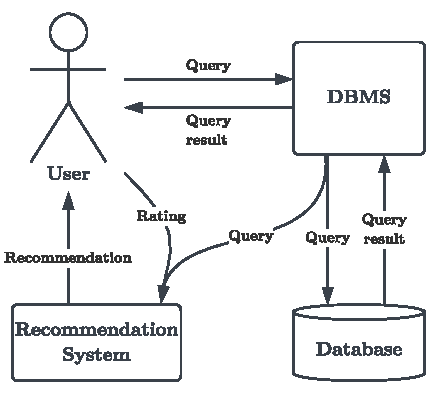
\includegraphics[width=0.30\textwidth]{imgs/architecture.pdf}
    \caption{\normalfont The workflow of the query recommendation system}
    \label{fig:workflow}
\end{figure}
\section{Solutions}
Multiple solutions are introduced in this part, starting with a preliminary naive approach and then refining it step by step to arrive at a definitive solution. The idea is to start with one of the traditional methods for handling recommendation systems and then improve it by combining it with many data mining techniques designed for handling massive amounts of data. 

\subsection{Naive solution}
\label{naive_solution}
Building a recommendation system based on the traditional methodologies is the easiest and most straightforward way to address the aforementioned problem; as was covered in the section on related work, the two primary approaches for these kinds of tasks are content-based and collaborative filtering. Considering that the input of the problem is an utility matrix partially filled with ratings and the remaining cells left blank, the choice fell in a first stage on collaborative filtering rather then content based, avoiding in this way to define item and user profiles. The choice of collaborative filtering gives the possibility to build either an Item-Item or a User-User collaborative filtering recommendation system, where the missing values — the cells $U_{ij}$ in the utility matrix that are blank — are filled according to one of the following schema:
\begin{enumerate}
    \item Item-Item collaborative filtering: this technique looks for the top $K$ queries that are most similar to query $j$ in the utility matrix. The average of the top-K items as rated by user $i$ is then used to fill the value for $U_{ij}$.
    \item User-User Collaborative Filtering: This method is similar to the previous one in concept, but differs slightly in that instead of looking for the top-K items that are similar to item $j$, this method looks for the top-K users that are similar to user $i$, and the value $U_{ij}$ is then filled with the average of the K most similar users to user $j$ that have rated item $j$. 
\end{enumerate}

Both these strategies requires to define a similarity measure to locate a neighborhood of K similar items or users. Due to a number of factors, which can be summed up as follows, the Item-Item approach was chosen over the User-user approach: 
\begin{itemize}
    \item Item's neighbourhood tends to change much slower in comparison to user's neighborhood. This is due to the fact that the user-user approach is good at making recommendations to users with unique tastes;
    \item Explainability of the model. In comparison to describing why a person has similar preferences to another, it is considerably simpler to explain the reasoning behind why an item has been recommended to a certain user based on previously rated goods; 
    \item Finding items of the same type is easier than finding users who only like items of a particular type, so item-item similarity frequently provides more reliable information;
    \item The systems considered in the aforementioned problem definition typically have more users than items, and the more users there are, the more expensive it will be to find the K closest neighbors. 
\end{itemize}

\subsubsection{Choosing a similarity measure}
\label{choosing_a_similarity_measure}
Finding a good similarity measure is crucial for making a solid neighborhood choice, but there are a few factors to take into account before choosing the best one. Two similarity measures — the Jaccard similarity and the Cosine similarity — were introduced in the section \ref{similatrity_measures} on similarity measures, one for sets (including binary vectors) and the other for vectors in euclidean space.
The optimal similarity measure for this problem is the cosine similarity, considering that neighborhood selection is based on item ratings corresponding to a column of the utility matrix i.e. a vector.
Even though the Jaccard similarity is not appropriate for handling vectors, a slightly modified version of this similarity measure is provided in the section for the next solution in order to handle vectors of user ratings. 

% pseudocode
\subsubsection{Pseudocode} The idea of Item-Item collaborative filtering is to iterate over all the utility matrix's cells. If a cell $U_{ij}$ is empty, it's rating is predicted by averaging the ratings of user $i$ for the $K$ queries that are most similar to query $j$. The similarity between two queries is given by the \emph{cos\_sim} procedure which takes as input two vectors to compare; the vector of the ratings of all the users for a single query $j$ is denoted as $U_{*j}$. In the pseudocode the neighborhood size $K$ is assumed to be $1$, i.e. the rating for $U_{ij}$ is predicted with the rating of user $i$ in the query that is most similar to query $j$.

\begin{algorithm}[h]
	\caption{Naive version of Item-Item collaborative filtering} 
	\begin{algorithmic}[1]
	    \For{$i \gets 1$ to $|S|$}  
	        \For{$j \gets 1$ to $|Q|$}
	            \If{$U_{ij} = \varnothing$} \Comment{Find empty cells $U_{ij}$}
	                \For{$q \gets 1$ to $|Q|$}  
        	            \State $\text{sim} \gets \text{sim} \cup \text{cos\_sim}(U_{*j}, U_{*q})$
                    \EndFor
                    \State $top \gets \argmax \,sim$ \Comment{Find most similar query}
                    \State $U_{ij} \gets top_i$
	            \EndIf
            \EndFor
        \EndFor
	\end{algorithmic} 
\end{algorithm}

This method involves computing the cosine similarity for each potential pair of queries. The cost of computing the cosine similarity is equal to the cost of computing the dot product of two queries, each of which corresponds to a column vector of $|S|$ components and has a cost of $O(|S|)$. The final cost to predict one single missing value of the utility matrix is given by $O(|S|\cdot|Q|^2)$. It's clear that predicting all the missing values of the utility matrix is costly, in particular when the dealing with a massive amount of users and queries.

\subsection{MinHash for LSH}
\label{minhash_section}
The primary issue with the previous solution is the algorithm's time complexity. In particular, the cost of finding the top $K$ queries that are similar to a given query is largely driven by the need for the algorithm to compute the similarity between all potential combinations of queries in the utility matrix. In order to address this issue, a more effective technique is presented in this section that employs minHash in conjunction with LSH to increase the similarity search's speed at the expense of accuracy. The purpose of LSH is to avoid checking the similarity between items that are definitely dissimilar and to concentrate solely on pairs of items that are likely to be similar; the latter are referred as \emph{candidate pairs}. Finding those candidate pairs in the original utility matrix is expensive; for this reason the idea is to apply LSH on a signature matrix rather than on the original utility matrix.

\subsubsection{MinHash} LSH typically operates on small signatures derived from a \emph{characteristic matrix}, which is a common representation of the data in order to describe the characteristic of the items. In the specific case of documents, the characteristic may be seen as a matrix $C$ with each row representing a potential word from a given vocabulary and each column representing a document: the word $i$ is present in the document $j$ if and only if $C_{ij} \neq 0$. There is a clear connection between the concept of characteristics matrix and the concept of utility matrix of recommendation systems, with the latter being a characteristics matrix in which each column $j$ is an item(a query) and each row $i$ corresponds to a user: the user $i$ has rated item $i$ if and only if $C_{ij} \neq 0$. This correlation between the twos clearly allows to exploit the MinHash technique to obtain a compressed representation of the utility matrix(from now on the utility matrix is considered to be the characteristic matrix). 

Dealing with the utility matrix directly is impractical in some cases due to its massive size; for this reason the idea is to replace the characteristics matrix with a compressed version called \emph{signature matrix} in such a way that the similarity of the items in the signature matrix is as close as possible to the similarity of items in the original characteristics matrix. No method can guarantee that the similarity will be exactly the same because some information from the characteristics matrix may be lost despite the fact that it was crucial in determining the similarity. The MinHash technique\cite{minhash} has been devised for the Jaccard similarity, thus as more signatures are added to the signatures matrix, the estimate of the Jaccard similarity between two items will get more accurate and similar to that for the original utility matrix.

The idea of MinHash is to generate a signature matrix $\delta$ by taking a number of $H$ of permutations $\pi$ of the rows of the utility matrix $U$(corresponding to the characteristics matrix) and finding for each of the items the first row in the permutation $\pi_t$ of $U_{*j}$ that has a value of one, i.e.
\begin{equation}
\begin{aligned}
\delta_{tj} \gets \text{min}_\pi (U_{\pi_tj} = 1)
\end{aligned}
\end{equation}



\paragraph{Example} Given a utility matrix $U$ of three items and a set of two permutations $\pi$, the signature matrix $\delta$ is produced as follows. 

\vspace{1em}
\begin{minipage}{0.3\linewidth}
    \centering
    $\pi=$
    \begin{tabular}{|l|l|l|}
    \hline
        \textbf{$\boldsymbol \pi_1$} & \textbf{$\boldsymbol \pi_2$} \\ \hline
        4 & 6 \\ \hline
        3 & 3 \\ \hline
        6 & 4 \\ \hline
        2 & 1 \\ \hline
        1 & 5 \\ \hline
        5 & 2 \\ \hline
    \end{tabular}
\end{minipage}
\begin{minipage}{0.3\linewidth}
    \centering
    $U=$
    \begin{tabular}{|l|l|l|}
    \hline
        \textbf{$\boldsymbol i_1$} & \textbf{$\boldsymbol i_2$} & \textbf{$\boldsymbol i_3$} \\ \hline
        1 & 1 & 1 \\ \hline
        0 & 1 & 1 \\ \hline
        1 & 0 & 0 \\ \hline
        0 & 0 & 0 \\ \hline
        0 & 1 & 1 \\ \hline
        1 & 0 & 1 \\ \hline
    \end{tabular}
\end{minipage}
\begin{minipage}{0.3\linewidth}
    \centering
    $\delta = $
    \begin{tabular}{|l|l|l|}
    \hline
        \textbf{$\boldsymbol i_1$} & \textbf{$\boldsymbol i_2$} & \textbf{$\boldsymbol i_3$} \\ \hline
        4 & 1 & 1 \\ \hline
        1 & 3 & 2 \\ \hline
    \end{tabular}
\end{minipage}


\subsubsection{Permutations generation} Generating the permutations and storing them in memory might be infeasible when dealing with utility matrices having a massive amount of users. For this reason a possibility is to simulate the effect of random perturbations by picking $H$ hash functions, one for each permutation, that return the index of a given row in the permutation. 

\begin{equation}
\begin{aligned}
\pi(x) = (ax + b) \bmod c
\end{aligned}
\end{equation}

where $a$, $b$ and $c$ are random value less than the number or users in the utility matrix, i.e $a, b, c \leq |S|$.

\subsubsection{Adapted MinHash for ratings} Given that the Jaccard similarity is defined for sets and consequently binary vector as exposed in Section \ref{similarity_measure_jaccard}, there is a problem in the above formulation of MinHash because it assumes that the characteristics matrix is made of 0s and 1s. However in the problem formulation, described in Section \ref{problem_statement}, the utility matrix $U$ is made of ratings in the range $[1,100]$. A solution for this problem is to convert the utility matrix $U$ containing the ratings into a matrix $\widehat{U}$ of zeros and ones, where the value $\widehat{U}_{ij} = 1$ indicates that the user $i$ has liked query $j$. Given that the threshold at which a query might be considered liked or not might vary depending on the situation, a threshold parameter named $T$ is introduced, according to which a query is considered liked if its rating is greater than $T$, i.e. 
\begin{equation}
\begin{aligned}
\widehat{U}_{ij} = 1 \iff U_{ij} \geq T
\end{aligned}
\label{eq_ratings}
\end{equation}
 
\paragraph{Example} Given a utility matrix $U$ of ratings in the range $[1,100]$, missing ratings denoted by cells with a value of $0$, and a threshold level of $T=50$ above which a rating is deemed to be positive, the corresponding utility matrix $\widehat{U}$ of positive ratings is obtained according to Eq. \ref{eq_ratings} as shown below. 

\vspace{1em}
\begin{minipage}{0.5\linewidth}
    \centering
    $U=$
    \begin{tabular}{|l|l|l|}
    \hline
        \textbf{$\boldsymbol q_1$} & \textbf{$\boldsymbol q_2$} & \textbf{$\boldsymbol q_3$} \\ \hline
        80 & 5 & 12 \\ \hline
        0 & 67 & 0 \\ \hline
        46 & 85 & 0 \\ \hline
        0 & 55 & 65 \\ \hline
        35 & 10 & 90 \\ \hline
        95 & 0 & 45 \\ \hline
    \end{tabular}
\end{minipage}
\begin{minipage}{0.5\linewidth}
    $\widehat{U}=$
    \begin{tabular}{|l|l|l|}
    \hline
        \textbf{$\boldsymbol q_1$} & \textbf{$\boldsymbol q_2$} & \textbf{$\boldsymbol q_3$} \\ \hline
        1 & 0 & 0 \\ \hline
        0 & 1 & 0 \\ \hline
        0 & 1 & 0 \\ \hline
        0 & 1 & 1 \\ \hline
        0 & 0 & 1 \\ \hline
        1 & 0 & 0 \\ \hline
    \end{tabular}
\end{minipage}

\vspace{1em}

The computation of the modified version of the utility matrix in practice is computationally expensive, in particular given $|S|$ and $|Q|$ respectively the number of users and the number of queries in the utility matrix, the cost of making such conversion is $O(|S| \cdot |Q|)$, which is quadratic in the size of the input. To overcome this issue a possibility is to use a slightly modified version of MinHash, denoted as \emph{MinHash with threshold}, that assigns to the signature matrix entry $\delta_{tj}$ the index of the first row in the permutation with a rating above the threshold level $T$.

\begin{equation}
\begin{aligned}
\delta_{tj} \gets \text{min}_\pi (U_{\pi_tj} \geq T)
\end{aligned}
\end{equation}

The resulting signature matrix is a good approximation for a modified version of the Jaccard similarity measure in order to take into account positive ratings as $1$ if they are greater than a threshold $T$ and $0$ the elements that are smaller than $T$. 

An implementation of this idea in pseudocode is shown in Algorithm \ref{minhash_alg}. The idea is to iterate over all queries and $H$ permutations of the utility matrix rows to discover the first row in the permuted order of the utility matrix that has a rating higher than the threshold $T$. In most cases, the loop of line 4 requires less iterations then the total number of users $|S|$ in the utility matrix.
The index $i$ is used as an input to create the permuted index $u$, increasing by one with each iteration until it reaches a maximum value of $|S|$. 

\begin{algorithm}[h]
    \caption{MinHash algorithm: signature matrix generation} 
    \begin{algorithmic}[1]
        \For{$j \gets 1$ to $|Q|$}
            \For{$h \gets 1$ to $H$}   
                \State $i \gets 1$ \Comment{$i$ is the original index of the rows}
                \While{$\delta_{hj} = \varnothing \cap i \leq |S|$} 
                    \State $u \gets \pi_h(i)$ \Comment{$u$ is the permutation of $i$}
                    \If{$U_{uj} \geq T$} 
                        \State $\delta_{hj} \gets i$
                    \EndIf
                    \State $i \gets i + 1$
                \EndWhile
            \EndFor
        \EndFor
    \end{algorithmic} 
    \label{minhash_alg}
\end{algorithm}

\subsubsection{Locality Sensitive Hashing} \label{lsh_description}
Once the signature matrix has been generated according to the modified version of MinHash with threshold $T$, the following step is to use the Locality Sensitive Hashing(LSH) technique to hash the queries in the signature matrix several times, in such a way that similar queries, i.e. queries with similar ratings, are more likely to be hashed to the same bucket than dissimilar queries are. The signature matrix is divided into $b$ bands, each made up of $r$ rows. Each band is then column-wise hashed into a set of buckets that is specific to that band, and queries that hashed to the same bucket are then considered to be candidate pairs. The information included in the candidate pairs can be used to reduce the time required to detect similar queries, so that each query $i$ is tested for similarity with each query $j$ that lie in the same bucket as query $i$ for at least one band, i.e. query $i$ and query $j$ are candidate pairs. 

The number of bands $b$ and the number of rows for each band $r$ play a crucial role in the amount of candidate pairs found for each query. In fact these two parameter are directly related one with the other i.e. recalling that $H$ is the number of permutation, namely the number of rows of the signature matrix $\delta$ then it holds that $b \cdot r = H$. Given this connection, it follows that the number of candidate pairs that LSH will find will increase if there are many bands and, as a result, few rows per band. On the other hand, if there are few bands and a large number of rows per band, LSH will locate fewer items that are similar to each other. A good trade-off must be chosen for the parameter $b$ defining the number of bands or equivalently for the parameter $r$ defining the number of rows for each band: the size of the signature matrix and the distribution of the data in the original utility matrix are two important criteria that must be taken into consideration while choosing these parameters; in the latter scenario, it is possible that all of the queries are extremely dissimilar from each other, which means that even a small value of $r$ is able to capture a significant number of candidate pairs. In the opposite scenario, it's possible that every query is incredibly similar to each other query, indicating that a low value of $r$ is insufficient and that the number of rows per band should be increased to prevent an excessive number of similar items from going against the goal of finding a good compromise on the number of similar items. 



\subsubsection{Making recommendations} \label{making_rec}
The final step is to provide recommendations using the item-item collaborative filtering method, similar to the one used in the Naive solution, with the exception that in this case, the iterative process that identifies the queries with the highest degree of similarity only iterates on the candidate pairs of a given query rather than on all possible queries. Considering time complexity, in the worst scenario the number of candidate pairs identified for each query is equal to the set of all the queries, leading the algorithm to fall back on the naive method. However this is just a limit case, in fact the number of candidate pairs can be reduced by appropriately adjusting the number of bands $b$ and the number of permutations $H$. 


\subsection{SimHash for LSH}
\label{simhash_section}
The Jaccard similarity, used with MinHash, is not the proper similarity measure for the problem taken into consideration; in fact, as discussed in section \ref{choosing_a_similarity_measure}, the Jaccard similarity is not the optimal similarity measure for vectors. In some situations, the modified version of the Jaccard similarity that takes the threshold parameter $T$ into account fails to measure the similarity between two queries. This situation occurs, for instance, when two queries have a rating that is remarkably similar, such as $49$ and $51$, but the threshold parameter $T=50$ makes them different. This problem is brought on by the indirect conversion of the utility matrix into a matrix of zeros and ones indicating whether a user liked or didn't like a query. A more suitable similarity metric for the issue under consideration in this study is the Cosine similarity, which can be computed on vectors of any type rather than only binary vectors.

This algorithm's general structure is quite similar to the one discussed for the solution with MinHash for LSH. The goal of the algorithm is to create a signature matrix $\delta$ that is representative of the original utility matrix, which means that given two general queries, their similarity should be preserved as much as possible in the signature matrix. The computation of the signature matrix should be quick and affordable, allowing the algorithm to benefit from using the signature matrix rather than the original utility matrix. After computing the signature matrix, the following step is to apply LSH to it in order to identify local similarities used to generated a set of candidate similar queries.


\subsubsection{SimHash intuition} The intuition behind of SimHash is to generate a signature matrix of $H$ rows, dividing the space containing the vectors corresponding to queries into $H$ hyperplanes passing through the origin. For any given hyperplane, each query ends up in one region of the hyperplane, either above or below the hyperplane. The signature matrix is filled for each query with its position with respect to the hyperplane $H_i$ corresponding to one row of the signature matrix $\delta$. The idea is that the closer two queries are, the more probable it is that they will be on the same region for a random hyperplane. For instance, on the majority of the planes that can be randomly generated, two queries that are relatively close to each other will end up in the same region.  The example in Figure \ref{fig:random_planes} accurately illustrates the intuition by demonstrating that for any arbitrary number of random hyperplanes and two similar queries $\vec{q_1}$ and $\vec{q_2}$, the probability of the queries falling on different sides of the hyperplanes is relatively small compared to the total number of hyperplanes: in that specific case, only the red plane divides the two queries into two different sides of the plane. SimHash has been demonstrated to be a locality-sensitive hash function that roughly approximates the cosine similarity\cite{simhash_demonstration} \cite{simhash_demonstration2}. 


\begin{figure}[h]
\begin{tikzpicture}[line cap=round,line join=round,>=triangle 45,x=1cm,y=1cm]
\begin{axis}[
    width=0.45*\textwidth,
    height=6.5cm,
    axis lines=middle,
    xmin=-10,
    xmax=10,
    ymin=-10,
    ymax=10,
    xtick={-10,-8,...,10},
    ytick={-10,-8,...,10},
    yticklabels={,,},
    xticklabels={,,}]
    
    \draw [-stealth, line width=1pt] (0,0) -- (6,8);
    \draw [-stealth, line width=1pt] (0,0) -- (8,6);
    \draw [line width=1pt,color=gray,domain=-100:100, dashed](-10,-2.776524) -- (10, 2.776524);
    \draw [line width=1pt,color=gray,domain=-100:100, dashed](-2.776524,-10) -- (2.776524, 10);
    \draw [line width=1pt,color=red,domain=-100:100, dashed](-10,-10) -- (10, 10);    
    \draw [line width=1pt,color=gray,domain=-100:100, dashed](-10,10) -- (10, -10);    
    \draw [line width=1pt,color=gray,domain=-100:100, dashed](2.776524,-10) -- (-2.776524, 10);
    \draw [line width=1pt,color=gray,domain=-100:100, dashed](-10, 2.776524) -- (10, -2.776524);

    \begin{scriptsize}
    \draw[color=black] (6,9) node {$\vec{q_1}$};
    \draw[color=black] (9,6) node {$\vec{q_2}$};
    \end{scriptsize}
\end{axis}
\end{tikzpicture}
\caption{\normalfont Two similar queries $\vec{q_1}$ and $\vec{q_2}$ are more likely to fall into the same region of any random hyperplane than when they are dissimilar.} 
\label{fig:random_planes}
\end{figure}

\subsubsection{Signature matrix computation} 
The computation of the signature matrix is straightforward based on the prior intuition: generate $H$ random hyperplanes and fill the ith row of the signature matrix with the query's position relative to the hyperplane. From a more formal perspective an \emph{hyperplane} is represented in a n-dimensional space with an n-dimensional vector that is orthogonal to the hyperplane. The position of a query vector $\vec{q_j}$ with respect to a general hyperplane $H_t$, represented by its orthogonal vector $\vec{h_t}$, is given by the sign of the projection of $\vec{q_j}$ on $\vec{h_t}$. Given that the projection of a vector on another one is computed using the dot product, the signature matrix cell corresponding to the ith hyperplane represented by its orthogonal vector $\vec{h_i}$ and the jth query $\vec{q_j}$ is computed as follows

\begin{equation}
\begin{aligned}
\delta_{tj} \gets \sign(\vec{h_t} \cdot \vec{q_j})
\end{aligned}
\end{equation}

where the $\sign$ function returns a value of $1$ if the argument that it takes as input is positive, otherwise it returns $-1$. The values of $1$ and $-1$, respectively, indicate that the query vector is located either on the positive or negative side of the hyperplane.
\begin{equation}
  \sign(\vec{h_t} \cdot \vec{q_j})=\begin{cases}
    1 & \text{if $\vec{h_t} \cdot \vec{q_j} \geq 0$}.\\
    0 & \text{otherwise}.
  \end{cases}
\label{sign_func}
\end{equation}

\paragraph{Example} Consider the example depicted in Figure \ref{fig:projection} of a generic hyperplane $H_1$ represented by its orthogonal vector $\vec{h_1} \in \mathbb{R}^2$ and two queries $\vec{q_1},\vec{q_2} \in \mathbb{R}^2$, characterized by the ratings given by two users. The position of the queries with respect to the hyperplane is determined by projecting $\vec{q_1}$ and $\vec{q_2}$ onto $\vec{h_1}$ and checking the sign, i.e. computing the sign of the dot product between the two vectors. In this specific instance, both queries are found to be on the positive side of the hyperplane $H_1$, therefore the corresponding cell in the signature matrix is filled with a value of $1$. Following the notation of signature matrix cell $\delta_{ij}$, defining the $ith$ row(the $ith$ hyperplane) and the $jth$ column(the $jth$ query) of the signature matrix, the signature for the first plane $H_1$ and the aforementioned queries is filled with $\delta_{11} \gets 1$ and $\delta_{12} \gets 1$.

\begin{figure}[h]
\begin{tikzpicture}[line cap=round,line join=round,>=triangle 45,x=1cm,y=1cm]
\begin{axis}[
    width=0.45*\textwidth,
    height=6.5cm,
    axis lines=middle,
    xmin=-42,
    xmax=45,
    ymin=-15,
    ymax=45,
    xtick={-40,-30,...,50},
    ytick={-10,0,...,50}]
    \clip(-41.94512591313005,-13.436694591890513) rectangle (57.578131814683154,49.31752666468061);
    \draw [-stealth, line width=1pt] (0,0) -- (30,25);
    \draw [-stealth, line width=1pt] (0,0) -- (10,40);
    \draw [line width=1.5pt,color=gray,domain=-100:100, dashed] plot(\x,{(-0--3.163372054762762*\x)/8.446133593990732});
    \draw [-stealth,color=gray, line width=1.5pt] (0,0) -- (-14.983685711606949,40.006110270862);
    \draw [mark=none, gray,thick, dotted] (-4.52,12.07)-- (30,25);
    \draw [mark=none, gray,thick, dotted] (-11.91,31.79)-- (10,40);
    \begin{scriptsize}
    \draw[color=black] (13,42) node {$\vec{q_1}$};
    \draw[color=black] (33,27) node {$\vec{q_2}$};
    \draw[color=black] (-12,20) node {$\vec{h_1}$};
    \draw[color=black] (-35,-9) node {$H_1$};
    \end{scriptsize}
\end{axis}
\end{tikzpicture}
\caption{\normalfont Projection of queries $\vec{q_1}$ and $\vec{q_2}$ onto $\vec{h_1}$ to find their position with respect to the hyperplane $H_1$.} 
\label{fig:projection}
\end{figure}




%% reprocessing, normalize the space 
\paragraph{Preprocessing} Given that a query in the utility matrix is represented by a vector of positive ratings with values between 1 and 100, all query vectors will always be located in the positive quadrant of the space. In the 2-dimensional example depicted in Figure \ref{fig:projection}, all the queries will always be located in the upper rightmost quadrant. This behavior is problematic because, regardless of the query, the projection on any hyperplane defined by an orthogonal vector falling within the aforementioned quadrant will always have a positive sign. To overcome this issue the solution is to normalize the utility matrix's ratings into the range $[-50,50]$ by subtracting the average value of $50$ from all the ratings in the utility matrix that are not $0$(missing rating), i.e. the new utility matrix $\widehat{U}$ is computed as follows:
\begin{equation}
\begin{aligned}
\widehat{U}_{ij} \gets U_{ij} - 50   && \forall i,j  \text{ s.t. } U_{ij} \neq 0
\end{aligned}
\end{equation}

The initial utility matrix $U$ is shown on the left in the example of Figure \ref{fig:standardization}, and the new utility matrix $\widehat{U}$, which is centered in $0$, is shown on the right. 



\begin{figure}[h]
    \begin{minipage}{0.49\linewidth}
        \centering
        \begin{tikzpicture}
        \begin{axis}[
                axis lines=middle,
                height=4.7cm, width=4.7cm,
                xmin=0,
                xmax=100,
                ymin=0,
                ymax=100,
                xtick={0,50,...,100},
                ytick={0,50,...,100}
                ]
            \pgfmathsetseed{7}%
            \addplot+[y filter/.expression={y},only marks,mark=*,draw=black, mark size=1.2pt, mark options={fill=gray},fill opacity=0.2,samples=40,domain=-0:100] {100*rnd};
        \end{axis}
        \end{tikzpicture}
    \end{minipage}
    \begin{minipage}{0.49\linewidth}
        \centering
        \begin{tikzpicture}
        \begin{axis}[
                axis lines=middle,
                height=4.7cm, width=4.7cm,
                xmin=-50,
                xmax=50,
                ymin=-50,
                ymax=50,
                xtick={-50,0,...,50},
                ytick={-50,0,...,50}
                ]
            \pgfmathsetseed{7}%
            \addplot+[y filter/.expression={y-50},only marks,mark=*,draw=black, mark size=1.2pt, mark options={fill=gray},fill opacity=0.2,samples=40,domain=-50:50] {100*rnd};
        \end{axis}
        \end{tikzpicture}
    \end{minipage}
    \caption{\normalfont The rating of the queries that originally are in the range $[1,100]$ are centered in the space to obtain ratings in $[-50,50]$.} 
    \label{fig:standardization}
\end{figure}


\paragraph{Pseudocode} Compared to the MinHash-based approach for producing the signature matrix, the SimHash algorithm is significantly simpler. Assuming that $H$ is a set of $|H|$ randomly generated hyperplanes, $\widehat{U}$ is the pre-processed utility matrix and $\sign$ is the function defined by Equation \ref{sign_func}, the signature matrix is computed as follows


\begin{algorithm}[h]
    \caption{SimHash algorithm: signature matrix generation} 
    \begin{algorithmic}[1]
        \For{$j \gets 1$ to $|Q|$}
            \For{$t \gets 1$ to $|H|$}   
                \State $\delta_{tj} \gets \sign(\widehat{U}_{*j} \cdot \vec{h_t})$
            \EndFor
        \EndFor
    \end{algorithmic} 
    \label{simhash_alg}
\end{algorithm}

\subsubsection{Making recommendations} Similar to the approach with MinHash, the next step is to leverage the signature matrix's information to find local similarities between queries using the Locality Sensitive Hashing technique outlined in Section \ref{lsh_description}. Given that not all candidate pairs correspond to similar queries, the candidate pairs need to be manually checked for similarity. According to the item-item collaborative filtering approach discussed in Section \ref{making_rec}, similar queries can be used to generate recommendations. The idea is to predict the rating of users $i$ to query $j$, which corresponds to $U_{ij}$ in the utility matrix, as the average of the ratings given by user $i$ for the $K$ queries that are most similar to query $j$. The complete architecture is shown in the diagram of Figure \ref{fig:cf_lsh}.
\begin{figure}[H]
    \centering
    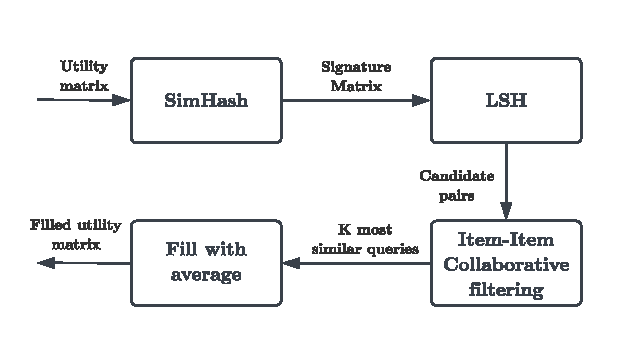
\includegraphics[width=0.43\textwidth]{imgs/cf_lsh_diagram.pdf}
    \caption{\normalfont Architecture of the collaborative filtering recommendation system using LSH to quickly identify related queries.}
    \label{fig:cf_lsh}
\end{figure}

\subsection{Content based recommendations}  \label{hybrid_rec_sys_solution}
Given that the similarity of queries is related to both their properties as well as their ratings given by users, it is possible for users to give the same ratings to two queries even when they are completely different. In light of this, the previous method — which combines collaborative filtering and LSH — is ineffective for providing relevant suggestions since it only took into account the ratings of queries rather than their structure.
Consequently, the idea is to combine the algorithm considered in the previous sections(LSH in combination with collaborative filtering) with a content-based strategy, to build an hybrid recommendation system. This new approach takes advantage of both the properties of the queries as well as the ratings given by the users to provide pertinent query recommendations based on previous user activity. The properties of a query can be interpreted from a conceptual or from a results-oriented point of view, respectively a query can be seen as a conjunction of conditions or as a collection of tuples. 

\subsubsection{Item and user profiles} Content-based recommendation systems look through item properties to find items that a specific user may be particularly interested in. This kind of recommendation system works on the principle of creating user and item profiles, one for each system user and one for each item, respectively. The principle is that after the profiles are created, it should be easy to calculate how much a user could appreciate an item: compare the user profile to that of the item, and if a high similarity is found, it is probable that the user would appreciate that item. 

\paragraph{Query profiles} An item profile should describe the important features of an item, for example in the case of movies, it might be the actors that are part of the movie. According to the same logic, the characteristics of a query, as previously noted, can be represented by its conditions or by the set of tuples it returns. In the instance examined in this work, the decision fell to take into account item profiles (referred to \emph{query profiles} throughout this paper) as the tuples returned by each query. The query profile for a generic query $j$, denoted as $IP_j$, is represented as vector with the same number of components as the total number of rows of the relational table. The $ith$ component of $IP_j$ is set $1$ if the query $j$ returned the $ith$ row of the relational table, otherwise $0$. For example the query profile of a generic query $j$ that returns only the first and the third row of a relational table with 5 rows can be represented as $IP_j = [1,0,1,0,0]$. 

\paragraph{User profiles} User profiles describe the user preference to the features of items profiles, for this reason to compare user profiles with query profiles, user profiles must have the same number of components of item profiles. Since each component of the user profile correspond to a row of the relational table, the issue becomes evident: In the utility matrix, the user's preferences are expressed on queries rather than the rows that the queries return, so it's not clear how to express the user preference of a single row. To solve this problem the solution is to find the rows returned by each query(simulating a DBMS) and then compute the preference of user $t$ to the $ith$ row of the relational table as the average rating given by user $t$ to all the queries returning the $ith$ row of the relational table. Throughout the article, the user profile for user $t$ is referred to as $UP_t$. 


\subsubsection{Hybrid recommendation system} 
Once user and query profiles have been appropriately generated, they can be used to match users with potentially interesting items. The approach is to calculate the cosine similarity between all the the vectorized user and item profiles in order to predict how much the user would likely appreciate an item. As already discussed in Section \ref{cosine_similarity} the cosine similarity measures the angle between two vector, so if the cosine similarity between an item profile $IP_j$ and a user profile $UP_t$ is high, it means that the angle between the two vectors is small, thus the user $t$ will probably like the query $j$. % However finding the potential matches between user profiles and query profiles involves computing the similarity between all the possible combinations of them, which is computationally expensive.
The idea, which is accurately depicted in Figure \ref{fig:hybrid}, is to build an \emph{Hybrid recommendation system} that combines the content-based approach introduced in this section with the collaborative filtering technique mentioned in the earlier solutions: the algorithm uses at first collaborative filtering with LSH to find the $K$ most similar queries of each query based on the user ratings in the utility matrix, then on top of that, the algorithm exploits content-based information derived from the queries to generate more accurate recommendations. As shown in figure \ref{fig:hybrid} the content-based phase attempts to match each user of the system with the optimal query among the $K$ most similar queries found by collaborative filtering: each user's profile is compared to the profile of each query among the $K$ that are most similar to a particular one. 

Similarly to the previous method, this one begins by running LSH with collaborative filtering. However, instead of predicting the missing ratings using the average of the $K$ most similar queries, it then runs content based to determine which query will be the best match for the user. 


\begin{figure}[h]
    \centering
    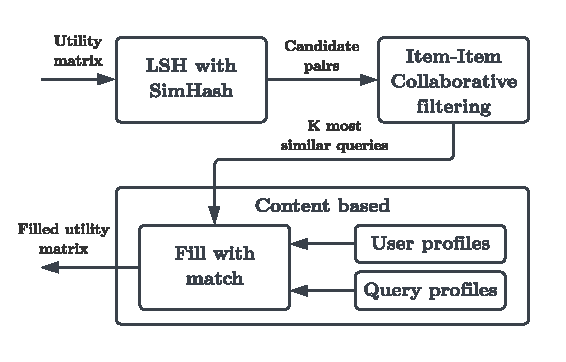
\includegraphics[width=0.43\textwidth]{imgs/hybrid_diagram.pdf}
    \caption{\normalfont Architecture of the hybrid recommendation system}
    \label{fig:hybrid}
\end{figure}




\subsection{Measuring the importance of a query(Part B)}

The aforementioned algorithm has been making recommendations based on queries that were already part of the query set, meaning that at least one user had submitted them. It's clear that in a more advanced scenario, queries that have not yet been posed to the DBMS might be of interest to the users of the system. Based on this, the purpose of this section is to provide a method for determining the importance of a query in general for all the users, i.e. how much the users of the system would like a query that may or may not have already been asked to the DBMS. 

Measuring the importance of a query must be done carefully and taking into account all the information that is available in the current system. For this reason there are several resources that can be helpful to build a system that computes the importance of a query; First of all there are two fundamental inputs:
\begin{itemize}
    \item the utility matrix filled with the missing ratings $(U)$
    \item the query itself, defined as a set of conditions $(q)$
\end{itemize}

The two aforementioned are the main inputs, but there are also some indirect inputs as a result of the utility matrix being calculated utilizing some other resources, namely the relational table $(R)$ and the query set $(Q)$. 

\begin{definition}[Importance]
For the purposes of this research, the \emph{importance} of a query has been defined in a way to assigns an integer value that is high if users in general will find that specific query interesting or a low value if users may think it is not significant at all. It was decided to use the convention of quantifying the importance of a query on a percentage scale that ranges from 0\% (not relevant) to 100\% (important).
\end{definition}


There are numerous approaches to finding a simple importance metric that could guarantee a precise enough measurement, but most of the time these approaches only use information from the relational table without considering the user's ratings, which is not enough when the objective is to deliver a sophisticated method that accurately measures the importance. The solution proposed in this section takes into account both the preferences of the users, expressed in terms of the utility matrix, and the factual utility of a query obtained by the rows that it returns from the relational table. Consequently, the suggested algorithm is divided into a preprocessing phase followed by two important steps: the first step computes the importance of a query based on the user ratings provided in the utility matrix, whereas the second one leverages the rows returned by the query, i.e. the result of a query.

\subsubsection{Preprocessing}
This early phase runs the query through the DBMS and produces results that allow some queries that could initially be considered as unimportant to be excluded from the subsequent phases. The idea is that queries returning all of the rows from the relational table $R$ or queries returning nothing at all should be treated as unimportant, and the algorithm should therefore assign them a low relevance rating, let's say $0\%$. This task usually takes very little time and is crucial because a query's outputs serve as its primary measure. 
This step is useful as generally a user would judge a query as a good one if it returns at least some outcomes, but not all the results. If the query is not labelled as unimportant in this preprocessing phase, the algorithm moves on with the next step.
\begin{algorithm}[h]
    \caption{Preprocessing} 
    \begin{algorithmic}[1]
        \State $rows \gets executeQuery(q)$
        \If{$rows = \varnothing$ or $rows = R$}
            \State $importance \gets 0\%$
        \Else
            \State $Step1()$
        \EndIf
    \end{algorithmic} 
    \label{alg:PartB_Preprocessing}
\end{algorithm}


\subsubsection{Step 1}

This step takes into consideration users' preferences provided by the utility matrix. The idea in this phase is to first obtain the average rating of each query from the utility matrix, by taking the average of each single column, corresponding to a query, and then compute the average rating given to each feature $f_i$ of that query as the average rating given by users to queries containing that feature $f_i$. In detail, as soon as each query $q_i$ is splitted into its conditions, the next step is to gather all of the features that shape each condition, without considering the value of that condition(recall that a feature is a relational table column, for example considering the condition $f_1 = Trento $ then $f_1$ is the feature and $Trento$ is the value). As each feature  $f_i$ is gathered, the algorithm gives to each feature $f_i$ a value of importance that is proportional to the average rating given by users to queries containing feature $f_i$. If a feature has no recorded grade, it will be counted as non important, so it will be assigned a 1\% grade. 

\paragraph{Example} Consider a feature \emph{city} which appears in only two queries of the query set, namely $q_1$ and $q_2$; suppose that according to the utility matrix the average ratings of query $q_1$ and $q_2$ are respectively $70$ and $90$. The average grade to the \emph{city} feature is computed as the average of $70$ and $90$, that is $80$.


\vspace{1em}
Once all the feature ratings are retrieved, the partial query importance(result of this first part) is computed as the average of its features' importance. To get this outcome the idea is to use the Geometric Mean\cite{geometric_mean} as the average measure of importance. The choice to use the Geometric Mean is driven by the necessity to give more emphasis to low rated features rather than highly rated features: given that a query is defined as a conjunction of condition, all the conditions must be satisfied in order for the query to return a specific row, thus even a negative grade on a single feature probably means that the entire query is not useful at all. 
The Algorithm \ref{alg:PartB_Step1} illustrates the pseudocode defining the process of computing the first partial importance, where the partial calculation of a query's importance computed in this first step is indicated as $I_a$. 

\begin{algorithm}[h]
    \caption{Step 1} 
    \begin{algorithmic}[1]
        \State $queryScore \gets []$
        \For{$j \gets 1$ to $|Q|$}\Comment{Avg rating of each query in Q}
            \State $queryScore_i \gets avg(U_{*j})$
        \EndFor
        \State
        \State $featureRating \gets []$
        \For{$f_i $ in $R.features$} \Comment{Avg rating of each feature in R}
            \State $featureScore \gets []$
            \For{$j \gets 1 $ to $ |Q|$}
                \If{$f_i$ in $q_j$}
                    \State $featureScore \gets featureScore \cup queryScore_j$
                \EndIf
            \EndFor
            \State $featureRating_{f_i} \gets avg(featureScore)$
        \EndFor 
        \State
        \State $queryFeatures \gets []$
        \For{$f_i $ in $R.features$} \Comment{Importance of the query q}
            \If{$f_i$ in $q$}
                \State $queryFeatures \gets queryFeatures \cup featureRating_{f_i}$
            \EndIf
        \EndFor
        \State $I_a \gets GeoMean(queryFeatures)$
    
    \end{algorithmic} 
    \label{alg:PartB_Step1}
\end{algorithm}


\subsubsection{Step 2}
In the previous step the importance of a query is calculated by the algorithm by solely taking into account the features in the query's conditions, without considering the values assigned to those features. This step instead is meant to take into consideration the values assigned to the features in order to obtain a more accurate measure of importance.

This step starts by computing the importance of the query as the importance of each of its valued-conditions. Differently from the previous phase, this step considers the value of the feature in the conditions, and computes the importance of each condition as the number of rows that satisfy that single condition. To give a reasonable grade to each condition, if the condition returns more than 20\% of the rows of the relational table, it will have a 100\% score, if 19\% it will have a score of 95\%, and so for steps of 5\% each time. The importance of the query is then given as the geometric mean of the importance of each condition that forms the query. The reason to do so is because if an item appears many times in the relational table, it means it is linked to many other objects inside the dataset, meaning it is connected to a lot of information. Then, the temporary score of the query will be an average of the score of each item.




% TODO: add gemetric mean equation 
%Geometric mean is used in the features importance, here it would penalize too much the query utility, I thnk normal average fits better


\paragraph{Example} Consider a query made only of two conditions, such as \emph{city = Trento} and \emph{age = 30}. The importance of the two conditions corresponds respectively to a number that is proportional to the number rows of the relational table having the value \emph{Trento} in the \emph{city} column and having the value \emph{30} in the age column. The final  importance is then given as the geometric mean of these two values.

\vspace{1em}

From this first score comes a major issue, which is the fact that if a query presents only one condition, its score will rely only on that condition's score, biasing its importance. Due to this, it is significant to find a way to penalize such a type of query, as in most cases they would be considered useless for all the stack of users.
There are many ways to weight an outcome based on the amount of conditions and probably the easiest one would be to multiply the importance value obtained so far by a weight factor given  by the number of conditions of the query $q$, denoted as $|q|$ divided by a parameter $\omega$ corresponding to the average number of conditions of the queries in the query set. This simple solution is formalized in Equation \ref{eq:easy_w}, however this method ends up penalizing too much all the middle range values.

\begin{equation}\label{eq:easy_w}
  I_b =  \frac{|q|}{\omega} \cdot I_b 
\end{equation}

For the aforementioned reason, the most proper way is instead to use a weight that correspond to the cumulative distribution function ($CDF$) of the exponential distribution, evaluated on the number of conditions of the query $q$. The $CDF$ of the exponential distribution is characterized by a rate parameter $\lambda$ which describes the increase rate of the $CDF$ function, i.e. a small value of $\lambda$ implies a slow asymptotic convergence of the function to the value of $1$.

\begin{equation}\label{eq:CDF_w}
    I_b = \left( 1 - e^{-\lambda \cdot \lvert q \lvert} \right) \cdot I_b 
\end{equation}

The Algorithm \ref{alg:PartB_Step2} illustrates the pseudocode defining the process of computing the second partial importance, where the partial calculation of a query's importance computed in this second step is indicated as $I_b$. 

\begin{algorithm}[h]
    \caption{Step 2} 
    \begin{algorithmic}[1]
        \State $itemScore \gets []$
        \ForAll{$c_i$ in $q$}   \Comment{Importance of each condition $c_i$ of q}
            \State $rows \gets exequteQuery(c_i)$
            \State $frac \gets \frac{|rows|}{|R|}$
            \If{$frac \geq 0.2$}
               \State $itemScore \gets 100$
            \Else
                \State $itemScore \gets 500 \cdot frac$ \Comment{ Note that here $frac < 0.2$}
            \EndIf
        \EndFor
        \State $I_b \gets GeoMean(itemScore)$
        \State $I_b \gets CDF(|q|) \cdot I_b$
    \end{algorithmic} 
    \label{alg:PartB_Step2}
\end{algorithm}

\subsubsection{Final Step}
The final value of importance for the query is given by the combination of two aforementioned steps. The idea is to give the rightful weight $\alpha$ to trade off the importance found by each step, emphasizing one over the other depending on the considered scenario. As data is different depending on the scenario, ideally it is better to have a variable weighted sum of the values of importance found in the two steps, rather than using always a constant value of $\alpha = 0.5$.
The final formulation to measure the query importance is defined as follows.
\begin{equation}\label{eq:QueryUtility_final}
    importance = \alpha \cdot  I_a + (1-\alpha) \cdot I_b
\end{equation}
The parameter $\alpha$, as well as $\lambda$ are two hyper-parameters of the formulation which should be tuned for each scenario, in particular it possible to find the optimal values relying on some kind of optimization technique.
\section{Experimental evaluation} 
\label{experimental_evalutation}
This part assess the solutions put forth in the preceding sections and demonstrate their efficacy in a simulated real-world scenario using data that was generated in a way that reflect reality. The performance of the algorithms explored in this paper have been measured on a machine with the following  specifications: Intel Core i7-6700HQ CPU @ 3.5GHz with 16 GB of RAM.


\subsection{Datasets}
The algorithms that implement the solutions proposed in this research have been tested on several datasets that were artificially constructed to as closely resemble a real-world scenario.
In particular, the synthetic dataset was produced starting with a relational table that was filled with the Scikit-Learn library's \emph{make\_blobs} function \cite{scikit-learn}, which makes it possible to generate correlated data. The choice of generating correlated data is motivated by the observation that in a real world scenario, in a relational table representing for example people, there exist groups of persons who share characteristics like eye color, height, etc. 

The query set is also built in a realistic manner; precisely, the conditions of each query are constructed by selecting a random number of features (even zero), giving each one a value in the feature's column with a chance of $99$ percent, and using the remaining probability to give a generic random value (even not in the admitted values of that feature). By doing this, the queries are created in a way that causes a great number of them to return some few rows, others to return all the rows, and eventually no rows at all. It's important to note that when a query has no conditions, all of the rows in the relational database are returned. 

The core of the dataset is the utility matrix and to generate this the idea is to create categories of users that tend to have the same taste of others. In addition users tends to act following patters. For this reason to fill the utility matrix ratings for the users the idea is to first split the users in three categories:
\begin{enumerate}
    \item $60$ percent of the users rates queries that returns similar rows in the same way. If two queries $q_1$ and $q_2$ returns the majority of the rows in common, the user who rates query $q_1$ with rating $r$ will rate query $q_2$ with a rating that differs by $r$ by a tiny factor $\gamma$, for instance $\gamma = 5$. 
    \item $30$ percent of users grade the queries proportionately with the amount of rows returned by the query. A user may be satisfied when the query returns some rows, but in another sense unsatisfied if the query does not return any row.
    \item the remaining $10$ percent of the users assign random ratings to the queries.
\end{enumerate}

Even though users can evaluate queries on a scale from $1$ to $100$, it is possible that two users will score a query differently in the real world. For example, one user may rate a query positively with a rating of 50, while another may rate the query positively with a rating of $100$. Because of this, the user ratings produced in the previous phase are randomly divided into the following categories: users who rate on a scale of $1$ to $50$, users who rate on a range of $50$ to $100$, $1$ to $100$, etc. Scaling the ratings is a straightforward process that may be carried out using equation \ref{scale_ratings}, where \emph{low} and \emph{high} represent the user's lowest and highest ratings, respectively.  


\begin{equation}
\begin{aligned}
    U_{ij} =  \frac{(\text{high} - \text{low})}{100}  U_{ij} + \text{low}
\end{aligned}
\label{scale_ratings}
\end{equation}




\subsubsection{Synthetic dataset characteristics}
The synthetic dataset is created as previously described using a relational table with $100$ features over a total of $10000$ rows, and in addition, the values of the relational table were filled with integer numbers; this latter choice is wise because, in general, relational tables take values from a specific domain, making representing cities by their names or by a representative integer number equivalent. The dataset is designed to simulate a system with $500$ users who have submitted the DBMS a total of $2000$ queries. Consequently, the utility matrix is composed of $500$ rows and $2000$ columns (queries). Last but not least, a script has been developed to calculate some crucial information from the relational database and the queries, revealing that, out of a total of $2000$ search queries, $721$ produced at least one row, and the average amount of rows returned by these queries is $3311$. 


Even if the numbers appear to be small, they are sufficient to evaluate the effectiveness of the proposed algorithms. They are particularly sufficient to demonstrate how the algorithm's performance improves in various scenarios: this dataset in particular was produced at that scale to enable its division into smaller portions for even more specific experiments. 

\subsubsection{Real dataset}
Relational tables typically contain experimental observations of real data; as a result, the solutions proposed in this work are also evaluated on a dataset in which a real relational table replaces the synthetic one. In this instance, the relational table is taken from the relational database of the 1994 Census Bureau \cite{relational_db}. This dataset is made up of $14$ columns that reflect individual attributes including age, sex, marital status, and income. The original dataset had over $50000$ individuals, however it was scaled down to only include $10000$ individuals in order to measure performance. The other components of the entire dataset are created using the same methodology as the synthetic one, yielding a total of $2000$ queries and $500$ users. In this case the dataset revealed that, out of a total of $2000$ search queries, $908$ produced at least one row, and the average amount of rows returned by these queries is $3649$. 


\subsection{Fast query similarity search with LSH}
\label{fast_sim_search}
This section analyzes the algorithm's initial building block to demonstrate how it performs in comparison to the baseline method for determining query similarity for collaborative filtering. This section specifically aims to demonstrate how the LSH approach, as explained in sections \ref{minhash_section} and \ref{simhash_section}, may significantly improve the naïve solution without LSH of section  \ref{naive_solution}. First, it is shown that using LSH with MinHash reduces the time required to find similar queries for collaborative filtering using the Jaccard similarity as a similarity measure for the queries, and second, it is shown that SimHash with LSH outperforms its corresponding baseline solution, which tries all possible combinations of queries to find the similar ones. Considering the original solutions, the goal of this section is to identify each query's most related queries based on the utility matrix ratings given by the users: without losing generality, the goal is slightly change to locate the most similar query rather than all the $K$ most similar ones. 

\subsubsection{LSH with MinHash}
In this section the LSH MinHash algorithm is compared with its naïve version that computes the Jaccard similarity to find the most similar query. The time efficiency of these two algorithms is compared in two different scenarios: the first involves a changing number of queries with a constant number of users, and the second involves a changing number of users having a constant number of queries. The approach is to divide the dataset used as input into smaller fractions and test the algorithms on those fractions, simulating smaller datasets in the process. In this case of MinHash and Jaccard similarity a dataset with at most $1000$ queries and $500$ users is sufficient to observe the time complexity growth. The plot of Figure \ref{fig:lsh_minhash_queries} reports the execution time of the two methods in a scenario with a constant amount of $500$ users and a variable number of queries. The other scenario is plotted in Figure \ref{fig:lsh_minhash_users} where the number of queries is kept constant at $1000$ queries and the number of users is variable. In both instances, MinHash is set up to generate a signature matrix with $200$ rows, corresponding to a total of $200$ random perturbations; additionally, the LSH bands are configured to have $6$ rows per band, which divides the signature matrix into $33$ bands. 

The two plots in Figures \ref{fig:lsh_minhash_queries} and Figure \ref{fig:lsh_minhash_users} clearly show the time improvements brought by the use of LSH as opposed to computing the similarity between every pair of queries. It is interesting to see that the two approaches perform similarly in the early stages with small datasets, but that one algorithm clearly outperforms the other in scenarios with larger datasets. 


\begin{figure}[h]        
    \begin{tikzpicture}
    \begin{axis}[
        xlabel=Number of queries,
        ylabel=Time (seconds),
        height=6cm,
        width = 0.5*\textwidth,
        grid = both,
        minor tick num = 1,
        major grid style = {lightgray},
        minor grid style = {lightgray!25},
        legend cell align = {left},
        legend pos = north west
    ]
    
    % Add values and attributes for the first plot
    \addplot[color=red,mark=*] coordinates {
    	(100, 1)
    	(200, 4)
    	(300, 9)
    	(400, 16)
    	(500, 25)
    	(600, 36)
    	(700, 48)
    	(800, 63)
    	(900, 80)
    	(1000, 100)
    };
    
    % Add values and attributes for the second plot
    \addplot[color=blue,mark=*] coordinates {
    	(100, 0)
    	(200, 0)
    	(300, 1)
    	(400, 1)
    	(500, 2)
    	(600, 3)
    	(700, 3)
    	(800, 4)
    	(900, 5)
    	(1000, 7)
    };
    
    \legend{Baseline solution Jaccard similarity,LSH with MinHash}
    \end{axis}
    \end{tikzpicture}
    
    \caption{\normalfont Time performance of the Naive algorithm compared with LSH using MinHash – Variable number of queries}
    \label{fig:lsh_minhash_queries}
\end{figure}

\begin{figure}[h]
    \begin{tikzpicture}
    \begin{axis}[
        xlabel=Number of users,
        ylabel=Time (seconds),
        height=6cm,
        width = 0.5*\textwidth,
        grid = both,
        minor tick num = 1,
        major grid style = {lightgray},
        minor grid style = {lightgray!25},
        legend cell align = {left},
        legend pos = north west
    ]
    
    % Add values and attributes for the first plot
    \addplot[color=red,mark=*] coordinates {
    	(100, 22)
    	(200, 41)
    	(300, 62)
    	(400, 80)
    	(500, 99)
    };
    
    % Add values and attributes for the second plot
    \addplot[color=blue,mark=*] coordinates {
    	(100, 3)
    	(200, 4)
    	(300, 3)
    	(400, 6)
    	(500, 6)
    };
    
    \legend{Baseline solution Jaccard,LSH with MinHash}
    \end{axis}
    \end{tikzpicture}
    \caption{\normalfont Time performance of the Naive algorithm compared with LSH using MinHash – Variable number of users}
    \label{fig:lsh_minhash_users}
\end{figure}



\subsubsection{LSH with SimHash}
The SimHash technique is compared in this section with its naïve counterpart, which computes the cosine similarity between all of the queries in the utility matrix. In this instance, it is possible to observe that leveraging LSH to identify similar queries enhances time performance of the algorithms. 

Given that the naïve approach using the Cosine similarity performs better than the technique using the Jaccard similarity, this time the algorithm is evaluated on a dataset with $2000$ queries rather than $1000$. Furthermore the number of hyperplanes for SimHash has been set at $200$ hyperplanes created at random, corresponding to $200$ rows of the signature matrix; the latter is divided into $13$ bands by LSH increasing the number of rows for each band to $15$. The decision to use a high number of rows per band is due to the fact that SimHash creates a signature matrix of zeros and ones, making it simpler for two queries in the same band to hash in the same bucket. Contrarily, MinHash's signature matrix is made up of integers between $1$ and the entire number of users in the system (rows of the utility matrix), making it less likely that two columns in the same band would hash into the same bucket. 

Similar to the previous instance, the LSH-based version of the method performs better than its naïve counterpart, which determines the similarity between all possible combinations of queries. The results are shown in Figures \ref{fig:lsh_simhash_queries} and Figure \ref{fig:lsh_simhash_users}, where the plots clearly show the comparison of the time performance of the two algorithms respectively as the number of queries and users increases.


\begin{figure}[h]        
        
    \begin{tikzpicture}
    \begin{axis}[
        xlabel=Number of queries,
        ylabel=Time (seconds),
        height=6cm,
        width = 0.5*\textwidth,
        grid = both,
        minor tick num = 1,
        major grid style = {lightgray},
        minor grid style = {lightgray!25},
        legend cell align = {left},
        legend pos = north west
    ]
    
    % Add values and attributes for the first plot
    \addplot[color=red,mark=*] coordinates {
    	(200, 1)
    	(400, 1)
    	(600, 3)
    	(800, 5)
    	(1000, 8)
    	(1200, 11)
    	(1400, 15)
    	(1600, 20)
    	(1800, 25)
    	(2000, 32)
    };
    
    % Add values and attributes for the second plot
    \addplot[color=blue,mark=*] coordinates {
    	(200, 0)
    	(400, 0)
    	(600, 0)
    	(800, 1)
    	(1000, 1)
    	(1200, 1)
    	(1400, 2)
    	(1600, 2)
    	(1800, 2)
    	(2000, 2)
    };
    
    \legend{Baseline solution Cosine similarity,LSH with SimHash}
    \end{axis}
    \end{tikzpicture}
    
    
    \caption{\normalfont Time performance of the Naive algorithm compared with LSH using SimHash – Variable number of queries}
    \label{fig:lsh_simhash_queries}
\end{figure}


\begin{figure}[h]        
        
    \begin{tikzpicture}
    \begin{axis}[
        xlabel=Number of users,
        ylabel=Time (seconds),
        ymax = 50,
        height=6cm,
        width = 0.5*\textwidth,
        grid = both,
        minor tick num = 1,
        major grid style = {lightgray},
        minor grid style = {lightgray!25},
        legend cell align = {left},
        legend pos = north west
    ]
    
    % Add values and attributes for the first plot
    \addplot[color=red,mark=*] coordinates {
    	(100, 26)
    	(200, 28)
    	(300, 29)
    	(400, 30)
    	(500, 32)
    };
    
    % Add values and attributes for the second plot
    \addplot[color=blue,mark=*] coordinates {
    	(100, 1)
    	(200, 2)
    	(300, 2)
    	(400, 2)
    	(500, 2)
    };
    
    \legend{Baseline solution Cosine similarity,LSH with SimHash}
    \end{axis}
    \end{tikzpicture}
    
    
    \caption{\normalfont Time performance of the Naive algorithm compared with LSH using SimHash – Variable number of users}
    \label{fig:lsh_simhash_queries}
\end{figure}



\subsubsection{LSH parameters tweaks} 
The parameters specifying the size of each LSH band and the number of rows of the signature matrix have a significant impact on LSH performance. Let's study these two characteristics independently in order to better understand their impact. 

\paragraph{Signature matrix rows} The algorithm's time performance will increase as the number of signature matrix's rows decrease, while the probability of finding the wrong most similar query, namely the \emph{error rate}, will decrease as the signature matrix gets smaller. Finding a good balance between the error rate and time performance is crucial, and in border cases it's possible that:
\begin{enumerate}
    \item the error rate is low, meaning the algorithm can accurately predict the queries' most similar queries. The issue with this border case is that LSH will likely discover a set of candidate similar pairs corresponding to all the combinations of queries, which means that the algorithm reverts to the naive approach of trying to find the query that is the most similar by comparing the similarities between all the possible pairs of queries. 
    \item time performance is the best, meaning the algorithm can find the most similar queries quickly. In this case the issue is related to the accuracy of the result, because with a tiny signature matrix, LSH will probably identify too few candidate similar pairs, which increases the likelihood that LSH will miss pairs of queries that may have been similar, i.e. the error rate is large.
\end{enumerate}

The result is clearly depicted in Figures \ref{fig:signature_matrix_rows_error_rate} and Figure \ref{fig:signature_matrix_rows_time} where the test was run using LSH with SimHash configured to divide the signature matrix in bands made of a constant number of $12$ rows. The time the algorithm took to discover the candidate similar queries as well as the error rate were recorded; the error rate is calculated as the complement of the accuracy, i.e. the fraction of successfully predicted most similar queries over all the other queries. 


\begin{figure}[h]        
    \begin{tikzpicture}
    \begin{axis}[
        xlabel=Signature matrix rows,
        ylabel=Error rate,
        height=6cm,
        width = 0.5*\textwidth,
        grid = both,
        minor tick num = 1,
        major grid style = {lightgray},
        minor grid style = {lightgray!25},
        legend cell align = {left},
        legend pos = north east
    ]
    
    \addplot[color=red,mark=*] coordinates {
    	(200, 0.758)
    	(400, 0.5385)
    	(600, 0.4325)
    	(800, 0.272)
    	(1000, 0.268)
    	(1200, 0.16600000000000004)
    	(1400, 0.10199999999999998)
    	(1600, 0.08799999999999997)
    	(1800, 0.0695)
    	(2000, 0.05500000000000005)
    };
    
    
    \legend{Error rate}
    \end{axis}
    \end{tikzpicture}
    
    \caption{\normalfont As the number of rows in the signature matrix rises, the error rate reduces.}
    \label{fig:signature_matrix_rows_error_rate}
\end{figure}


\begin{figure}[h]        
    \begin{tikzpicture}
    \begin{axis}[
        xlabel=Signature matrix rows,
        ylabel=Execution time(seconds),
        height=6cm,
        width = 0.5*\textwidth,
        grid = both,
        minor tick num = 1,
        major grid style = {lightgray},
        minor grid style = {lightgray!25},
        legend cell align = {left},
        legend pos = north west
    ]
    
    \addplot[color=blue,mark=*] coordinates {
    	(200, 6)
    	(400, 13)
    	(600, 17)
    	(800, 25)
    	(1000, 26)
    	(1200, 31)
    	(1400, 37)
    	(1600, 38)
    	(1800, 40)
    	(2000, 42)
    };
    
    \legend{Execution time}
    \end{axis}
    \end{tikzpicture}
    
    \caption{\normalfont The time required to search for the most similar query grows as the signature matrix's row count rises.}
    \label{fig:signature_matrix_rows_time}
\end{figure}


\paragraph{LSH band size} As already anticipated also in Section \ref{lsh_description} choosing a good number of rows per band or similarly a number of bands that divides the signature matrix are crucial. In particular in the same way shown for the number of rows of the signature matrix it's possible to observe that testing LSH with SimHash configured to have a constant amount of $200$ signature rows(number of hyperplanes for SimHash) and a variable number of rows per band, when the number of rows for each band increase:
\begin{enumerate}
    \item the error rate tend to increase as shown in Figure \ref{fig:rows_per_band_error_rate}; this is a consequence of the fact that the number of candidate pairs found by LSH decrease.
    \item the algorithm will take less time to find the most similar query as show in Figure \ref{fig:rows_per_band_time}. This is also caused by the fact that LSH only finds a small number of candidate similar pairs of queries, and thus the time required to compare all the possible candidate pairs is less.
\end{enumerate}



\begin{figure}[h]        
    \begin{tikzpicture}
    \begin{axis}[
        xlabel=LSH rows for each band,
        ylabel=Error rate,
        height=6cm,
        width = 0.5*\textwidth,
        grid = both,
        minor tick num = 1,
        major grid style = {lightgray},
        minor grid style = {lightgray!25},
        legend cell align = {left},
        legend pos = north west
    ]
    
    \addplot[color=red,mark=*] coordinates {
        (5, 0.001)
        (6, 0.013)
        (7, 0.023499)
        (8, 0.1915)
        (9, 0.3595)
        (10, 0.497)
        (11, 0.6355)
        (12, 0.864)
        (13, 0.8305)
        (14, 0.895)
        (15, 0.897)
    };
    
    
    \legend{Error rate}
    \end{axis}
    \end{tikzpicture}
    
    \caption{\normalfont As the size of each band rises, the error rate increases.}
    \label{fig:rows_per_band_error_rate}
\end{figure}


\begin{figure}[h]        
    \begin{tikzpicture}
    \begin{axis}[
        xlabel=LSH rows for each band,
        ylabel=Execution time(seconds),
        height=6cm,
        width = 0.5*\textwidth,
        grid = both,
        minor tick num = 1,
        major grid style = {lightgray},
        minor grid style = {lightgray!25},
        legend cell align = {left},
        legend pos = north east
    ]
    
    \addplot[color=blue,mark=*] coordinates {
        (5, 46)
        (6, 41)
        (7, 40)
        (8, 28)
        (9, 20)
        (10, 15)
        (11, 10)
        (12, 4)
        (13, 4)
        (14, 3)
        (15, 3)
    };
    
    \legend{Execution time}
    \end{axis}
    \end{tikzpicture}
    
    \caption{\normalfont The time required to search for the most similar query decreases as the size of each band increases.}
    \label{fig:rows_per_band_time}
\end{figure}


As seen in this section, it is crucial to properly adjust the hyperparameters before executing the algorithm. This should be done while taking into account all possible scenarios. The measurements in this section are calculated by iterating over the various value combinations, measuring the time performance of the process step-by-step, and determining the error as the opposite of accuracy. 

\subsection{Accuracy of the recommendation system}
\label{accuracy_of_rec_sys}
The preceding section analyzed the runtime performance of the algorithm using only collaborative filtering with LSH while tweaking the LSH parameters. However, time performance is not the only aspect that defines a recommendation system's quality. In this section, the accuracy of the algorithms described in this paper is measured using two fundamental metrics: \emph{mean absolute error}(MAE) and \emph{root mean square error}(RMSE). The idea is to compare the accuracy on the following versions of the algorithm:
\begin{enumerate}
    \item Collaborative filtering recommendation system with LSH using MinHash discussed in Section \ref{minhash_section}. 
    \item Collaborative filtering recommendation system with LSH using SimHash discussed in Section \ref{simhash_section}. 
    \item Hybrid recommendation system that combines collaborative filtering(using LSH) with a content based approach as discussed in Section \ref{hybrid_rec_sys_solution}.
    \item Random recommendation system that randomly fills the ratings in the utility matrix.
\end{enumerate}

\subsubsection{MAE and RMSE} The mean absolute error and the root mean squared error have been selected as the two metrics to evaluate the model's accuracy. The distinction between the two is that whereas root mean square error measures the average squared difference between the expected and actual ratings, mean absolute error measures the average difference between the predicted and actual ratings. A high value of RMSE or MAE indicates poor performance in terms of the quality of the recommendation system: both should be lowered to have the maximum accuracy. 

\begin{minipage}{0.49\linewidth}
    \centering
    \begin{equation}
    \label{rmse}
    \begin{aligned}
        MAE = \frac{\sum_i^n \lvert y_i  x_i \lvert }{n}
    \end{aligned}
    \end{equation}
\end{minipage}
\begin{minipage}{0.49\linewidth}
    \centering
    \begin{equation}
    \label{rmse}
    \begin{aligned}
        RMSE = \sqrt{\frac{\sum_i^n (y_i  x_i)^2 }{n}}
    \end{aligned}
    \end{equation}
    
\end{minipage}

\subsubsection{K-fold cross validation}
The idea for measuring the quality of the recommendations, is to apply the K-fold cross validation approach, which takes a portion of non-zero ratings from the utility matrix to be used as a test set, and then runs the aforementioned algorithms on the utility matrix with the ratings in the test set removed. This total procedure is executed $K$ times, where $K=10$ has been selected as a suitable value for the number of folds. The average of the two metrics' accuracy throughout the several folds provides the final indication of MAE and RMSE accuracy. Similar results were obtained using the K-folding approach on both the real dataset and the synthetic dataset, indicating the increase in accuracy that follows from using the content-based strategy of Section \ref{hybrid_rec_sys_solution} to create a hybrid recommendation system. The histograms of Figures \ref{fig:rmse_histo} and \ref{fig:mae_histo} in particular show the average result of the accuracy metrics mentioned above applied on each fold of both the real and synthetic datasets. 

The figures make it clear that the random recommendation system's RMSE and MAE are high in both the datasets, suggesting poor prediction accuracy. The collaborative filtering method is definitely better than the random method, and as the plots demonstrate, the accuracy of the recommendation system increases further when it is combined with a content-based method to form a hybrid recommendation system. The latter is driven by the fact that user ratings are not the only criteria for identifying queries that may be of interest to a user: other aspects of the queries such as the rows they return(their content), are also very important in identifying queries that may be of use to a particular user. 


\begin{figure}[h]        
    \begin{tikzpicture}
        \begin{axis}[
            enlargelimits=0.15,
            x tick label style={
            /pgf/number format/1000 sep=},
            ylabel={\small{RMSE}},
            width = 0.5*\textwidth, 
            height = 6cm,
            legend pos=north west,
            symbolic x coords={CF + LSH(MinHash), CF + LSH(SimHash), Hybrid, Random},
            xtick=data,
            tick label style={font=\scriptsize},
            ybar,
            bar width = .6cm,
            grid = both,
            minor tick num = 1,
            major grid style = {lightgray},
            minor grid style = {lightgray!25},
            legend cell align = {left},
            legend pos = north west
        ]
        
        \addplot coordinates {(CF + LSH(MinHash),25.390739) (CF + LSH(SimHash),25.575141) (Hybrid,19.596540) (Random,41.166241)};
        \addplot coordinates {(CF + LSH(MinHash),25.248578) (CF + LSH(SimHash),25.365404) (Hybrid,18.864845) (Random,41.073583)};
        
        \legend{Synthetic,Real}
        \end{axis}
    \end{tikzpicture}
    
    \caption{\normalfont Average RMSE of the different algorithms on the two datasets.}
    \label{fig:rmse_histo}
\end{figure}


\begin{figure}[h]        
    \begin{tikzpicture}
        \begin{axis}[
            enlargelimits=0.15,
            x tick label style={
            /pgf/number format/1000 sep=},
            ylabel={\small{MAE}},
            width = 0.5*\textwidth, 
            height = 6cm,
            legend pos=north west,
            symbolic x coords={CF + LSH(MinHash), CF + LSH(SimHash), Hybrid, Random},
            xtick=data,
            tick label style={font=\scriptsize},
            ybar,
            bar width = .6cm,
            grid = both,
            minor tick num = 1,
            major grid style = {lightgray},
            minor grid style = {lightgray!25},
            legend cell align = {left},
            legend pos = north west
        ]
        
        \addplot coordinates {(CF + LSH(MinHash),19.932730) (CF + LSH(SimHash),20.168860) (Hybrid,13.415692) (Random,33.618878)};
        \addplot coordinates {(CF + LSH(MinHash),19.796775) (CF + LSH(SimHash),20.022409) (Hybrid,12.450330) (Random,33.535856)};
        
        \legend{Synthetic,Real}
        \end{axis}
    \end{tikzpicture}
    
    \caption{\normalfont Average MAE of the different algorithms on the two datasets.}
    \label{fig:mae_histo}
\end{figure}



It's interesting to note that, for all of the algorithms mentioned above, with the exception of the hybrid algorithm, the accuracy metrics produce results that are identical on both datasets, whereas the hybrid recommendation system appears to produce results that are more accurate on the real dataset. This might be related to the data distribution governing the two datasets.


\subsection{Observations}
A recommendation system's quality is determined by a number of essential aspects, including time performance and accuracy. Thanks to the experiments conducted in this section, it is possible to conclude that as model accuracy rises, time performance decreases, and vice versa:
\begin{itemize}
    \item With the random recommendation method, the recommendations are easily calculated and it takes less than one second to fill the utility matrix. However, this approach has the drawback of providing useless recommendations that are driven by randomness.
    \item When LSH and collaborative filtering are combined together, the recommendation system is more accurate compared to random recommendations, however this comes at the expense of a little higher overhead in terms of time performance. In addition, as demonstrated in Section \ref{fast_sim_search}, SimHash should be preferred over MinHash on big datasets since it allows for a faster execution time while maintaining the same accuracy for the recommendations: as shown in Section \ref{accuracy_of_rec_sys}, the accuracy of the two LSH techniques is roughly equivalent. 
    \item The collaborative filtering approach relies solely on information derived from user ratings, without considering the characteristics of the queries. This has motivated the integration of a content-based approach with the already-existing collaborative filtering recommendation system described in Section \ref{simhash_section} in order to increase the accuracy of the recommendations. The experiments conducted in Section \ref{accuracy_of_rec_sys} demonstrate the accuracy improvement and prove that the hybrid recommendation system works better than the approach employing simply collaborative filtering. However this comes at a higher cost to pay in terms of execution time, in fact computing the item and user profiles is costly and may require several minutes compared to the few seconds needed for collaborative filtering.
\end{itemize}



\section{Conclusion}

The solutions presented and examined in this research produced satisfactory results, demonstrating how the integration of several data mining approaches may result in an advanced recommendation system that can make meaningful recommendations. The final algorithm was built one block at a time, producing two distinct algorithms: the first one based on collaborative filtering with LSH, which keeps both a high accuracy and good time performance, and a second solution, which integrates content based to the previous solution to build an hybrid recommendation system with an even greater accuracy but worse time performance. The experiments conducted in Section \ref{experimental_evalutation} demonstrate how combining a content-based approach with the a collaborative filtering method results in a hybrid recommendation system that generates recommendations that are more accurate. Furthermore it was also possible to demonstrate that standard methodologies, such as the Naive algorithm using only collaborative filtering of Section \ref{naive_solution}, are inapplicable in the case of large datasets, but that combining various strategies, as seen in LSH, can result in solutions that enable dealing with massive datasets. To sum up, this research made it possible to discover that the problem of providing useful query recommendations in the context of DBMS is a very challenging task that depends on a wide range of factors. 


In conclusion, the research presented in this paper has demonstrated the effectiveness of the proposed query recommendation system in addressing the specific problem addressed. However, as with any new system, there is still much work to be done in terms of implementation and fine-tuning. In particular, future work could focus on implementing the solution using the map-reduce framework: this would allow for more efficient and scalable processing of large datasets, which is crucial for the success of query recommendation systems. Additionally, it would be valuable to investigate the possibility of integrating the proposed solution with other technologies to enhance its overall performance

%%
%% The next two lines define the bibliography style to be used, and
%% the bibliography file.
\bibliographystyle{ACM-Reference-Format}
\bibliography{bibliography}

%%
%% If your work has an appendix, this is the place to put it.
\appendix

\end{document}
\endinput
%%
%% End of file `sample-sigconf.tex'.


